\section{NLP-based Configuration Completion}

We leverage the regularity of configurations to design an intelligent
configuration completion engine.
According to Hindle et al.~\cite{naturalness}, regularities in texts
can be easily exploited by natural language processing (NLP) techniques.
Hence, we use n-grams, ranked based on likelihood, to complete
the next token(s) in a configuration.
%Inspired by them, we decided to use N-grams as a basis of our model. This
%effectively makes all router configuration histories a part of the search
%space for our model. 

Prior to building the model, we employ a networking-specific optimization
inspired by our observation that IP prefixes are often unique to devices
(Section~\ref{sec:similarity}): we replace prefixes with generic {\tt PREFIX}
tokens. As we show below, this allows us to accurately
predicate the next token in configuration statements involving prefixes.

%In particular, we use an
%n-gram model to generate predictions using likelihood estimators to score our
%n-grams. In particular, we made use of bigrams and trigrams, the latter of
%which performed consistently better. We preprocessed the data and added
%placeholders for certain tokens like IP addresses, subnet masks, and interface
%names

%\begin{figure}
%	\centering
%	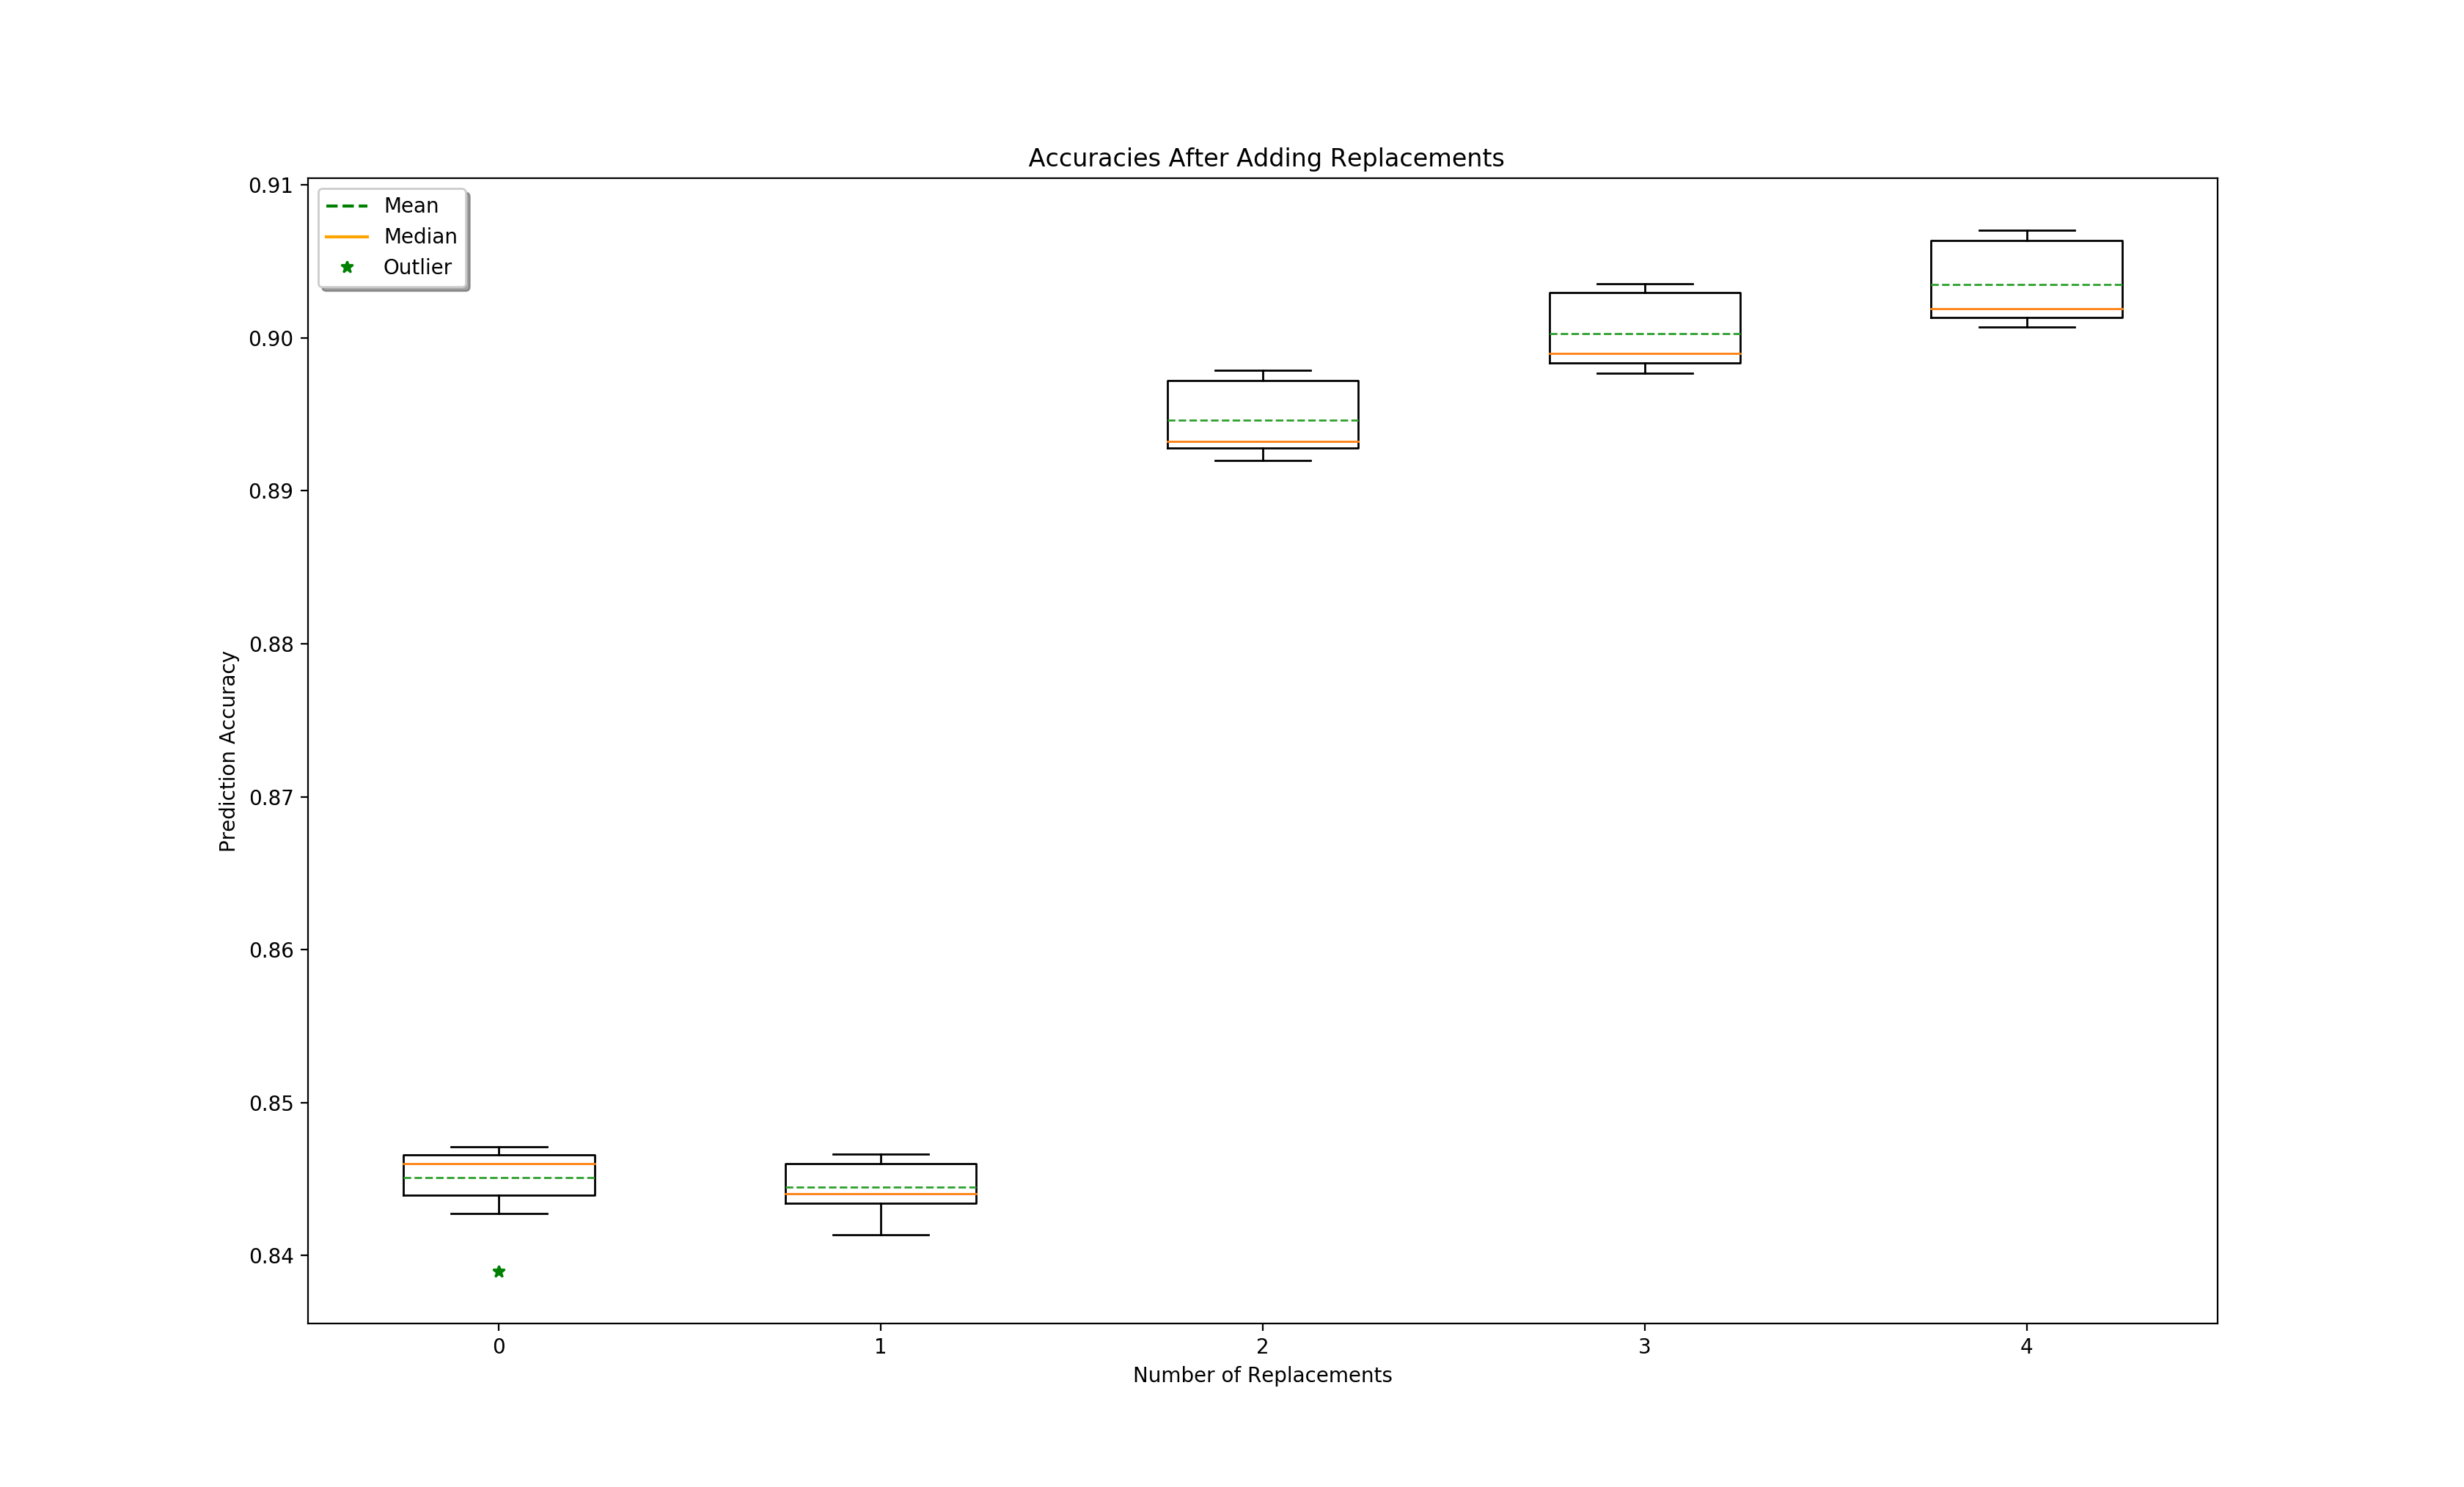
\includegraphics[width=\columnwidth]{replacement_analysis.png}
%	\caption{Accuracy increase as we utilize placeholders to replace noisy tokens}
%    \label{fig:replacement_analysis}
%\end{figure}

{\bf Preliminary Results.} We applied our framework to Cisco configurations of
core, border, and distribution routers from three large university networks
(Table~\ref{tab:datasets}). To test the accuracy of our model, we perform
leave-one-out cross validation: one (set of) configuration(s) is used for
testing and the remainder are used for training. We ``rebuild'' the test
configuration(s) token-by-token by using our n-gram model to predict the next
token based on the  prior n-1 tokens; we do not predict across lines. A
prediction is marked as successful when the actual next token in the
configuration is within the top three results generated by the model. 
%Our initial analyses showed that the engine was trying to predict what the
%user would enter after a complete configuration statement. This greatly
%affected our accuracies, and thus we altered our model to only suggest tokens
%that appear on the same line.  The table below and
%(Figure~\ref{fig:config_sizes}) give some statistics about the
%configurations.

\begin{table}
    \small \centering
    \begin{tabular}{ | c | c | c | c |}
    \hline
        {\bf Univ.} & {\bf No. of Configs} & {\bf Total Lines} & {\bf Avg
    Lines} \\ 
    \hline
    A & 35 & 73K & 2.1K \\ 
    B & 26 & 61K & 2.3K \\ 
    C & 24 & 67K & 2.8K \\ 
    \hline
    \end{tabular}
    \caption{Configurations used in our evaluation}
    \vspace{-1em}
    \label{tab:datasets}
\end{table}

%\begin{figure}
%	\centering
%	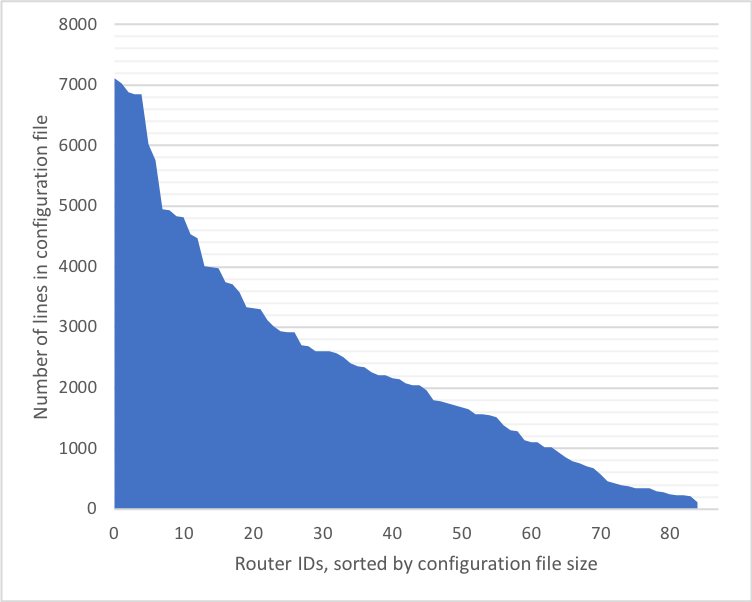
\includegraphics[width=\columnwidth]{config_sizes.png}
%	\caption{Size distribution of all configuration files}
%    \label{fig:uni_analysis}
%\end{figure}

Figure~\ref{fig:uni_analysis}, shows the prediction accuracy for
the routers in each network. Our approach achieves a high prediction accuracy
($>$85\%) for the majority of routers. Without our placeholders optimization,
this accuracy is 5\% lower.

\begin{figure}
    \centering
	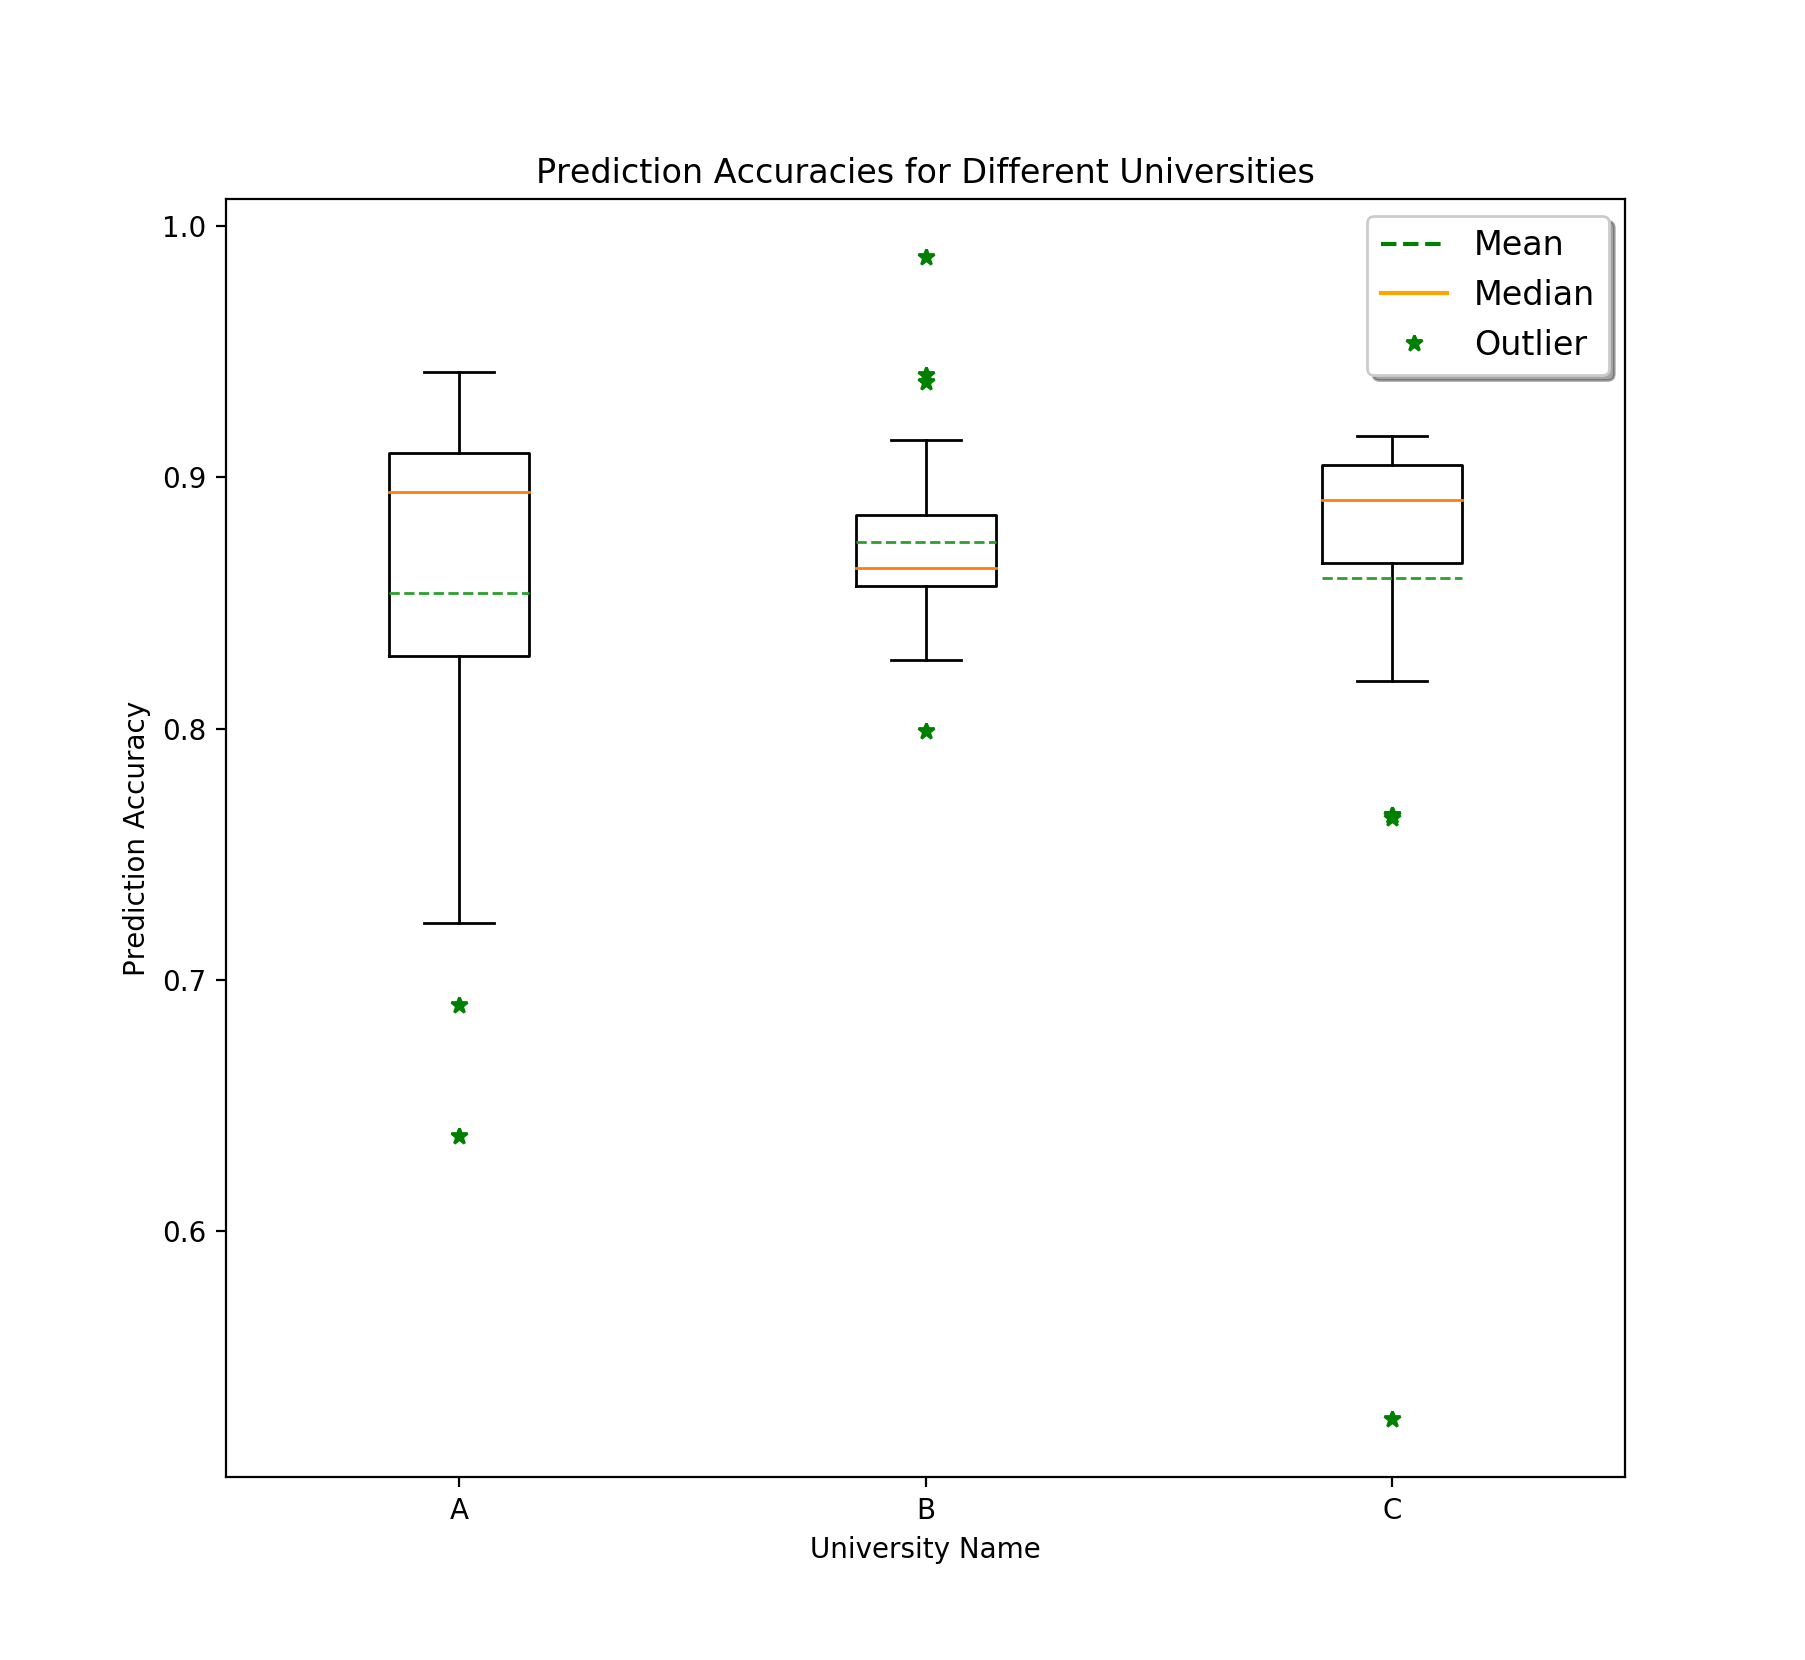
\includegraphics[width=0.6\columnwidth]{uni_analysis.png}
	\caption{Prediction accuracy per-router per-network}
    \vspace{-1em}
    \label{fig:uni_analysis}
\end{figure}

We also analyzed the effects of training on more configurations in time and
space. As shown in Figure~\ref{fig:monthly_analysis}, our framework does not
require a long history of configurations to achieve reasonable accuracy. In
contrast, training on more devices results in higher accuracies
(Figure~\ref{fig:device_analysis}). However, training on more devices has
diminishing returns, because additional devices play the same role as
existing devices, and hence are very similar.

%which did not seem to have a
%statistically relevant effect on our accuracies. We also varied the number of
%devices considered for our training set (Figure~\ref{fig:device_analysis}).
%This helped us assess our model's performance when we considered devices with
%different roles. 
%Additionally, our analyses showed that our preprocessing helped reduce a
%significant amount of noise from the data, where we saw a 5\% increase in
%accuracy through placeholders alone. The majority of this increase came
%through generalizing IP addresses and subnet masks.

\begin{figure}
	\centering
	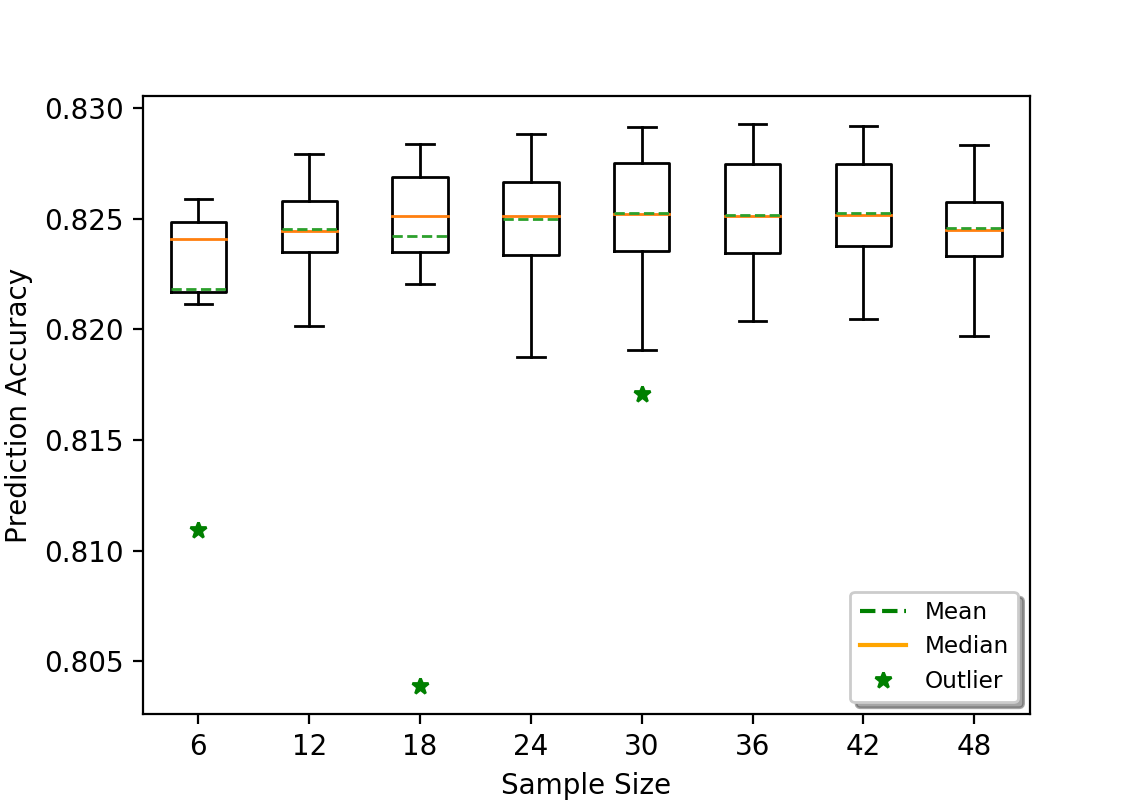
\includegraphics[width=0.6\columnwidth]{monthly_analysis.png}
	\caption{Impact of number of months for Univ-A}
    \vspace{-1em}
    \label{fig:monthly_analysis}
\end{figure}
\begin{figure}
	\centering
	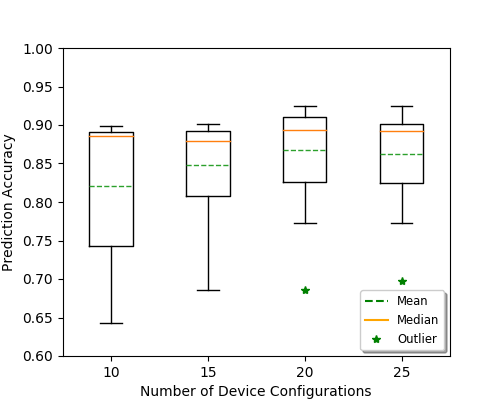
\includegraphics[width=0.6\columnwidth]{device_analysis.png}
	\caption{Impact of number of devices for Univ-A}
    \vspace{-1em}
    \label{fig:device_analysis}
\end{figure}

\section{Future Work}

Our analyses help direct our attention towards areas of improvements for the model. The variance seen in our device analysis suggests that having different models for router of different "roles" could help improve prediction accuracies. Additionally, we plan on exploring the possibility of using larger n-grams to suggest complete statements. Lastly, we hope to evaluate our model against the current state of the art: tab-completion in CLIs on modern routers.
